\subsection{External interfaces requirements}

\subsubsection{User interfaces}
\paragraph{\ac{eMSP}}
The \ac{eMSP} should be accessible through an application installed on the mobile device.
The first interface shown to the user, if not already done, is the \textit{login} page where the user has to input the email and password in order to authenticate.
From the \textit{login} page there is also the possibility to go to the \textit{sign up} page where the fields for inserting the necessary information are shown.
After logging in, there are multiple tabs in the app, which are:
\begin{itemize}
    \item A satellite map of the charging stations near user's position;
    \item A personalizable ranked list based on parameters chosen by the user (distance, price, environmental friendliness\ldots).
    \item A screen for enabling/disabling suggestions from the system and for setting up the connection to the user web calendar.
\end{itemize}
By selecting a station (from the ranked list or the satellite map) the specific information about it are shown. The user can select the date and the time slot from the available ones.

A \ac{CPO} can register to the system with a special form providing Company name, email, password and \gls{partita IVA}. Once the \ac{CPO} is registered and logged in, he can insert/remove the \ac{API} reference to the interface of a \ac{CPMS}.

\paragraph{\ac{CPMS}}
The \ac{CPMS} works as a web application; When a \ac{CPO}maintainer logs in he has the possibility to handle all the added stations.\\
In particular he can view: the system status, the list of charging stations and their policy, the available sockets and the \ac{SoC} of batteries.\\
The \ac{CPO}maintainers can change the policy of each charging station; in particular they can:
\begin{itemize}
    \item Choose a the energy provider from a list of \acp{DSO};
    \item Choose to use only the energy stored in the batteries and, once discharged, to go into automatic mode;
    \item Choose the automatic mode, that will pick autonomously which \ac{DSO} to use, whether to use batteries and when to recharge them;
\end{itemize}

The \ac{CPO} can also view the price of his service and set the revenue percentage for a single charge. Finally, the \ac{CPO} can also create some special offers.

\subsubsection{Hardware interfaces}
\paragraph{\ac{eMSP}}
The user, in order to interact with the \ac{eMSP}, must have a device that is provided with a \ac{GPS} and internet connection. Thanks to this, the user can search for close charging stations, see if those are available and can book or cancel a charge.
A Bluetooth peripheral should also be available to the user when he is in the vehicle, in order to make a connection with it. Thanks to this the device can query the vehicle infos (such as average battery consumption per kilometer, estimated autonomy and \ac{SoC}) so that the system can suggest to the user when and where to charge the vehicle.

\paragraph{\ac{CPMS}}
In order to use the \ac{CPMS}, the \ac{CPO}maintainer (the only type of user of this system) should have a personal computer with internet connection available so that it's possible to see the system info and communicate changes to the system (i.e. change the energy source of a charging station or setting the new revenue for a charge).

\subsubsection{Software interfaces}
\paragraph{\ac{eMSP}}
In order to provide all the functionalities, the \ac{eMSP} should provide the following software interfaces:
\begin{itemize}
    \item Register to the \ac{eMSP} as a user providing name, email, password, birthday, payment info;
    \item Register to the \ac{eMSP} as a \ac{CPO} providing name, email, password, \gls{partita IVA};
    \item Confirm the registration of a given user;
    \item Login to the \ac{eMSP} providing correct email and password;
    \item Retrieving data about charging stations, such as the nearest (providing a location), the cheapest or a list of K charging stations;
    \item Book a charge providing charging station, time slot and type of charge;
    \item Cancel an already booked charge;
    \item Paying a charge with the already set payment method;
    \item A \ac{CPO} can add a \ac{CPMS} providing a link to its \ac{API} interface;
\end{itemize}

\paragraph{\ac{CPMS}}
The \ac{CPMS} should provide to the external world interfaces for:
\begin{itemize}
    \item Login to the \ac{CPMS} providing an ID and a password;
    \item Enable a charge on a charging station, passing the ID (a PIN in order to authorize the charge once the user gets in the station), the station and the time slot;
    \item Get information of a particular charging station (location, price of the charge, parameter of environmental friendliness, type of charges available);
    \item Get the availability state of a particular socket;
    \item Get the future availability of the sockets managed by the system;
\end{itemize}

\subsubsection{Communication interfaces}
\paragraph{\ac{eMSP}}
The \ac{eMSP} should use internet connection in order to interact with the back-end of the system, query the different \acp{CPMS} and be connected to the electronic calendar. In order to communicate with the vehicle the user device should also be provided with bluetooth so that can retrieve data from the vehicle and use that for suggesting when and where to charge the vehicle.

\paragraph{\ac{CPMS}}
The \ac{eMSP} should be provided with a local connection in order to link all the infrastructure and make it manageable by a user in the local connection.
An internet connection should also be present in order to make the system reachable by the external world; in particular it is needed for queries and external functions made by users (like booking a charge, canceling a charge, seeing what time slots are available) and in order to manage remotely the system from the \ac{CPO}maintainers.

\subsection{Functional requirements}

\begin{enumerate}[label=\textbf{R\arabic*}]
    \item The \ac{eMSP} shall allow the users to register, providing name, surname, birthday, email, password, payment method;\label{req:eMSP-user-registration}
    \item The \ac{eMSP} shall allow the user to login with email and password;\label{req:eMSP-user-login}
    \item The \ac{eMSP} shall provide information about a selected station such as types of available sockets, price for the charge, location, available time slots, parameter on environmental friendliness;\label{req:eMSP-info-station}
    \item The \ac{eMSP} shall reserve a socket in the right charging station for a user who booked a charge through the application;\label{req:eMSP-reserve-socket}
    \item The \ac{eMSP} shall allow only one user to book a socket in a particular time slot, so no booking collisions shall occur;\label{req:eMSP-no-book-collisions}
    \item The \ac{eMSP} shall allow the user to pay for a booked charge;\label{req:eMSP-payment}
    \item The \ac{eMSP} shall refund the user when a charge is canceled;\label{req:eMSP-refund}
    \item The \ac{eMSP} shall allow the user to see nearby\footnote{This parameter may be set by the user} charging stations ordered by distance, price or environmental friendliness;\label{req:eMSP-see-stations}
    \item The \ac{eMSP} shall be able to connect to a web calendar, retrieve information about the appointments and parse them;\label{req:eMSP-connect-calendar}
    \item The \ac{eMSP} shall be able to use the information about the appointments, the charging stations and the vehicle in order to proactively suggest to the user when and where to charge the vehicle;\label{req:eMSP-proactive-suggestions}
    \item The \ac{eMSP} shall notify the user when the charging process is finished;\label{req:eMSP-notification}
    \item The \ac{eMSP} shall aggregate different \acp{CPO};\label{req:eMSP-compatible}
    \item The \ac{eMSP} shall allow a \ac{CPO} to register, providing name, email, password, \gls{partita IVA};\label{req:eMSP-cpo-registration}
    \item the \ac{eMSP} shall allow to add to an already registered \ac{CPO} a \ac{CPMS}, providing its \ac{API} reference;\label{req:eMSP-add-cpms}
    \item The \ac{eMSP} shall verify the correctness of the identification data for the \acp{CPO};\label{req:eMSP-correct-cpo-info}
    \item The \ac{eMSP} shall allow the \ac{CPO} to set the wanted revenue percentage;\label{req:eMSP-set-revenue}
    \item The \ac{eMSP} shall allow the \ac{CPO} to set special offers;\label{req:eMSP-set-special-offers}
    \item The \ac{CPMS} shall be reachable by \acp{eMSP} in order to perform or cancel a booking, or query the system;\label{req:CPMS-reachable}
    \item The \ac{CPMS} shall allow the \ac{CPO}maintainer to access to the system;\label{req:CPMS-accessible}
    \item The \ac{CPMS} shall allow the \ac{CPO}maintainer to modify the information about their systems, such as adding/removing charging stations, set stations sources and create/remove maintainers;\label{req:CPMS-modify-cpo-infos}
    \item The \ac{CPMS} shall allow the \ac{CPO}maintainer to choose the energy source and strategy;\label{req:CPMS-select-source-strategy}
    \item The \ac{CPMS} shall allow the \ac{CPO}maintainer to choose manual or automatic mode;\label{req:CPMS-select-mode}
\end{enumerate}

\begin{table}[h]
    \begin{center}
        \begin{tabular}{|c||c|c|c|c|c|}
            \hline
            Requirements/Goals:                   & \ref{goal:eMSP-helps-selecting} & \ref{goal:eMSP-booking-charge} & \ref{goal:eMSP-allow-charge} & \ref{goal:CPMS-handles-charge} & \ref{goal:CPMS-manage-station} \\\hline\hline
            \ref{req:eMSP-user-registration}      & X                               & X                              & X                            &                                &                                \\\hline
            \ref{req:eMSP-user-login}             & X                               & X                              & X                            &                                &                                \\\hline
            \ref{req:eMSP-info-station}           & X                               &                                & X                            &                                &                                \\\hline
            \ref{req:eMSP-reserve-socket}         &                                 & X                              & X                            &                                &                                \\\hline
            \ref{req:eMSP-no-book-collisions}     &                                 & X                              & X                            &                                &                                \\\hline
            \ref{req:eMSP-payment}                &                                 & X                              &                              &                                &                                \\\hline
            \ref{req:eMSP-refund}                 &                                 & X                              &                              &                                &                                \\\hline
            \ref{req:eMSP-see-stations}           & X                               & X                              &                              &                                &                                \\\hline
            \ref{req:eMSP-connect-calendar}       & X                               & X                              &                              &                                &                                \\\hline
            \ref{req:eMSP-proactive-suggestions}  & X                               & X                              &                              &                                &                                \\\hline
            \ref{req:eMSP-notification}           &                                 &                                & X                            &                                &                                \\\hline
            \ref{req:eMSP-compatible}             &                                 & X                              &                              &                                &                                \\\hline
            \ref{req:eMSP-cpo-registration}       &                                 & X                              &                              & X                              &                                \\\hline
            \ref{req:eMSP-add-cpms}               &                                 & X                              &                              & X                              &                                \\\hline
            \ref{req:eMSP-correct-cpo-info}       &                                 & X                              &                              & X                              &                                \\\hline
            \ref{req:eMSP-set-revenue}            &                                 &                                &                              &                                & X                              \\\hline
            \ref{req:eMSP-set-special-offers}     &                                 &                                &                              &                                & X                              \\\hline
            \ref{req:CPMS-reachable}              & X                               & X                              & X                            & X                              &                                \\\hline
            \ref{req:CPMS-accessible}             &                                 &                                &                              & X                              & X                              \\\hline
            \ref{req:CPMS-modify-cpo-infos}       &                                 &                                &                              &                                & X                              \\\hline
            \ref{req:CPMS-select-source-strategy} &                                 &                                &                              & X                              & X                              \\\hline
            \ref{req:CPMS-select-mode}            &                                 &                                &                              & X                              & X                              \\\hline
        \end{tabular}
    \end{center}
    \caption{Linking table among goals and requirements}
\end{table}

\clearpage
\subsubsection{Use cases}
% \begin{table}[h]
%     \begin{center}
%         \begin{tabular}{|c||p{10cm}|}
%             \hline
%             Actor: & \\
%             \hline
%             Entry conditions: &  \\
%             \hline
%             Event flow: & 
%             \begin{enumerate}
%                 \item 
%             \end{enumerate}
%             \\
%             \hline
%             Exit condition: &  \\
%             \hline
%             Exceptions: &
%             \begin{itemize}
%                 \item 
%             \end{itemize}
%             \\
%             \hline
%         \end{tabular}
%     \end{center}
%     \caption{}
% \end{table}


% Unregistered user
\begin{table}[h]
    \begin{center}
        \begin{tabular}{|c||p{10cm}|}
            \hline
            Actor:            & User                                               \\
            \hline
            Entry conditions: & The user doesn't have any account on the platform. \\
            \hline
            Event flow:       &
            \begin{enumerate}
                \item The user presses the \textit{Register} button;
                \item The user enters name, surname, birthday, email, password, payment method;
                \item The user presses the confirmation button;
                \item The system sends a confirmation email to the provided email address;
                \item The user presses a link in the confirmation email;
                \item The system shows a success message.
            \end{enumerate}
            \\
            \hline
            Exit condition:   & The user now has an active account.                \\
            \hline
            Exceptions:       &
            \begin{itemize}
                \item The user takes more than 15 minutes to press the confirmation email: In this case the account won't be created, the system will notify the user and all the process should be redone;
                \item The user inserts an already registered email to the system: the system notifies the user without letting the process continue;
                \item The user doesn't insert some required information: the system notifies the user without letting the process continue.
            \end{itemize}
            \\
            \hline
        \end{tabular}
    \end{center}
    \caption{Unregistered user}
\end{table}

% Unregistered CPO
\begin{table}[h]
    \begin{center}
        \begin{tabular}{|c||p{10cm}|}
            \hline
            Actor:            & \ac{CPO}                                        \\
            \hline
            Entry conditions: & The \ac{CPO} isn't registered yet.              \\
            \hline
            Event flow:       &
            \begin{enumerate}
                \item The \ac{CPO} selects the \textit{Register as \ac{CPO}} option;
                \item The \ac{CPO} enters company name, email, password and \gls{partita IVA};
                \item The system sends a confirmation email to the provided email address;
                \item The \ac{CPO} presses a link in the confirmation email;
                \item The system shows a success message.
            \end{enumerate}
            \\
            \hline
            Exit condition:   & The \ac{CPO} is now registered to the platform. \\
            \hline
            Exceptions:       &
            \begin{itemize}
                \item The \ac{CPO} takes more than 15 minutes to press the confirmation email: In this case the account won't be created, the system will notify the \ac{CPO} and all the process should be redone;
                \item The \ac{CPO} inserts an already registered email to the system: the system notifies the \ac{CPO} without letting the process continue;
                \item The \ac{CPO} doesn't insert some required information: the system notifies the \ac{CPO} without letting the process continue;
                \item The \gls{partita IVA} isn't valid or can't be verified: the system notifies the \ac{CPO} without letting the process continue.
            \end{itemize}
            \\
            \hline
        \end{tabular}
    \end{center}
    \caption{Unregistered \ac{CPO}}
\end{table}

% User/CPO logs in
\begin{table}[h]
    \begin{center}
        \begin{tabular}{|c||p{10cm}|}
            \hline
            Actor:            & User or \ac{CPO}                                                                                                                                                                                                                                                                                             \\
            \hline
            Entry conditions: & The actor is not already logged in.                                                                                                                                                                                                                                                                          \\
            \hline
            Event flow:       &
            \begin{enumerate}
                \item The actor presses the login button;
                \item The actor inserts email and password;
                \item The system validates the credentials;
                \item The system lets the actor access the available features.
            \end{enumerate}
            \\
            \hline
            Exit condition:   & The actor is logged into the system and can perform some specific actions (i.e. for the user: search near stations, book a charge, cancel a charge, pay for a charge and view previously booked charges; for the \ac{CPO}: add a \ac{CPMS}, remove a \ac{CPMS}, set revenue percentage, set special offers). \\
            \hline
            Exceptions:       &
            \begin{itemize}
                \item The user inserts wrong credentials: The system notifies it with an error message.
            \end{itemize}
            \\
            \hline
        \end{tabular}
    \end{center}
    \caption{User or \ac{CPO} logs in}
\end{table}

% CPO adds a CPMS
\begin{table}[h]
    \begin{center}
        \begin{tabular}{|c||p{10cm}|}
            \hline
            Actor:            & \ac{CPO}                                                                                         \\
            \hline
            Entry conditions: & The \ac{CPO} is already logged in the system.                                                    \\
            \hline
            Event flow:       &
            \begin{enumerate}
                \item The \ac{CPO} selects the option to add a \ac{CPMS};
                \item The \ac{CPO} inserts the \ac{API} reference in the form and sends it;
                \item The system checks if it exists and if it is reachable;
                \item The system adds the \ac{CPMS} to the available \acp{CPMS} and retrieves all the charging stations attached to the \ac{CPMS}.
            \end{enumerate}
            \\
            \hline
            Exit condition:   & A \ac{CPMS} is added to the system and can be reached to book charges or other queries by users. \\
            \hline
            Exceptions:       &
            \begin{itemize}
                \item The API reference doesn't exist, the \ac{CPMS} isn't reachable or the \ac{CPMS} was already added to the system previously: the system returns an error message with the specific reason.
            \end{itemize}
            \\
            \hline
        \end{tabular}
    \end{center}
    \caption{\ac{CPO} adds a \ac{CPMS} to the system}
\end{table}

% CPO sets the revenue percentage
\begin{table}[h]
    \begin{center}
        \begin{tabular}{|c||p{10cm}|}
            \hline
            Actor:            & \ac{CPO}                                                     \\
            \hline
            Entry conditions: & The \ac{CPO} is already logged into the system.              \\
            \hline
            Event flow:       &
            \begin{enumerate}
                \item The \ac{CPO} selects the option to insert the wanted revenue percentage for a charge performed on a charging station owned by the \ac{CPO};
                \item The \ac{CPO} inputs the wanted revenue percentage;
                \item The system checks the inputted value;
                \item The system shows a successful message.
            \end{enumerate}
            \\
            \hline
            Exit condition:   & The revenue percentage is changed to the new inputted value. \\
            \hline
            Exceptions:       &
            \begin{itemize}
                \item The value inserted is not a positive value (i.e. the value is below 0\%): the system returns an error message.
            \end{itemize}
            \\
            \hline
        \end{tabular}
    \end{center}
    \caption{A \ac{CPO} sets the revenue percentage}
\end{table}

% CPO sets a special offer
\begin{table}[h]
    \begin{center}
        \begin{tabular}{|c||p{10cm}|}
            \hline
            Actor:            & \ac{CPO}                                        \\
            \hline
            Entry conditions: & The \ac{CPO} is already logged into the system. \\
            \hline
            Event flow:       &
            \begin{enumerate}
                \item The \ac{CPO} selects the option to create a special offer for his charging stations;
                \item The \ac{CPO} sets the various parameters of the offer, such as validity period and discount;
                \item The system verifies the validity of the parameters set;
                \item The system shows a successful message.
            \end{enumerate}
            \\
            \hline
            Exit condition:   & There is a new special offer in the system.     \\
            \hline
            Exceptions:       &
            \begin{itemize}
                \item The values inserted aren't valid: the system returns an error message.
            \end{itemize}
            \\
            \hline
        \end{tabular}
    \end{center}
    \caption{A \ac{CPO} sets a special offer}
\end{table}

% User gets nearby charging stations
\begin{table}[h]
    \begin{center}
        \begin{tabular}{|c||p{10cm}|}
            \hline
            Actor:            & User                                            \\
            \hline
            Entry conditions: & The user is already logged into the system.     \\
            \hline
            Event flow:       &
            \begin{enumerate}
                \item The user presses the \textit{Map} button;
                \item The user inserts the location and time frame;
                \item The user presses the \textit{Search} button;
                \item The system shows a ordered list of k best nearby stations.
            \end{enumerate}
            \\
            \hline
            Exit condition:   & The user has a list of ordered nearby stations. \\
            \hline
            Exceptions:       &
            \begin{itemize}
                \item The inserted time frame isn't correct: the system returns an error message.
            \end{itemize}
            \\
            \hline
        \end{tabular}
    \end{center}
    \caption{The user searches for nearby stations}
\end{table}

% User books a charge
\begin{table}[h]
    \begin{center}
        \begin{tabular}{|c||p{10cm}|}
            \hline
            Actor:            & User                                                                                    \\
            \hline
            Entry conditions: & The user is already logged into the system and he has already searched for the station. \\
            \hline
            Event flow:       &
            \begin{enumerate}
                \item The user inserts the time frame;
                \item The user presses the \textit{Book} button;
                \item The system checks the time frame;
                \item The system shows the charge ID and sends the user an email with the details.
            \end{enumerate}
            \\
            \hline
            Exit condition:   & The user has now a booked charge.                                                       \\
            \hline
            Exceptions:       &
            \begin{itemize}
                \item The inserted time frame isn't correct: the system returns an error message;
                \item The inserted time frame is not available: the system returns an error message.
            \end{itemize}
            \\
            \hline
        \end{tabular}
    \end{center}
    \caption{User books a charge}
\end{table}

% User pays for a charge
\begin{table}[h]
    \begin{center}
        \begin{tabular}{|c||p{10cm}|}
            \hline
            Actor:            & User                                                                                       \\
            \hline
            Entry conditions: & The user is already logged into the system and there is an already existing booked charge. \\
            \hline
            Event flow:       &
            \begin{enumerate}
                \item The user presses the \textit{Pay} button near the booked charge;
                \item The system asks for a confirmation;
                \item The user presses the \textit{Confirm} button;
                \item The system checks the charge existence and ownership;
                \item The system performs the payment, marks the charge as enabled and sends a confirmation email.
            \end{enumerate}
            \\
            \hline
            Exit condition:   & A booked charge is paid.                                                                   \\
            \hline
            Exceptions:       &
            \begin{itemize}
                \item The charge does not exist: the system returns an error message;
                \item The charge does not belong to the user: the system returns an error message;
                \item The payment fails: the system returns an error message.
            \end{itemize}
            \\
            \hline
        \end{tabular}
    \end{center}
    \caption{User pays for a charge}
\end{table}

% User cancels a charge
\begin{table}[h]
    \begin{center}
        \begin{tabular}{|c||p{10cm}|}
            \hline
            Actor:            & User                                                                                       \\
            \hline
            Entry conditions: & The user is already logged into the system and there is an already existing booked charge. \\
            \hline
            Event flow:       &
            \begin{enumerate}
                \item The user presses the \textit{Cancel} button near the booked charge;
                \item The system asks for a confirmation;
                \item The user presses the \textit{Confirm} button;
                \item \item The system checks the charge existence and ownership;
                \item The system cancels the charge and in case of an already paid one, it refunds the user;
                \item The system sends a confirmation email.
            \end{enumerate}
            \\
            \hline
            Exit condition:   & A previously booked charge is canceled.                                                    \\
            \hline
            Exceptions:       &
            \begin{itemize}
                \item The charge does not exist: the system returns an error message;
                \item The charge does not belong to the user: the system returns an error message.
            \end{itemize}
            \\
            \hline
        \end{tabular}
    \end{center}
    \caption{User cancels a charge}
\end{table}

% User performs a charge
\begin{table}[h]
    \begin{center}
        \begin{tabular}{|c||p{10cm}|}
            \hline
            Actor:            & User                                           \\
            \hline
            Entry conditions: & The user has already booked and paid a charge. \\
            \hline
            Event flow:       &
            \begin{enumerate}
                \item The user plugs the charging connector into the vehicle;
                \item The user inserts the charge ID into the Charging Socket;
                \item The charging socket verifies the charge ID and the presence of the charging connector;
                \item The charging socket starts the charge;
                \item The charging socket sends the user an email when the charging process is done.
            \end{enumerate}
            \\
            \hline
            Exit condition:   & The vehicle is charged.                        \\
            \hline
            Exceptions:       &
            \begin{itemize}
                \item The charge ID is not valid: the charging socket displays an error message;
                \item The charging connector is not connected: the charging socket displays an error message.
            \end{itemize}
            \\
            \hline
        \end{tabular}
    \end{center}
    \caption{User charges vehicle}
\end{table}

% System suggests charge via calendar
\begin{table}[h]
    \begin{center}
        \begin{tabular}{|c||p{10cm}|}
            \hline
            Actor:            & eMall                                                       \\
            \hline
            Entry conditions: & The user smartphone is connected via bluetooth  to the car. \\
            \hline
            Event flow:       &
            \begin{enumerate}
                \item The system acquires the car position;
                \item The system acquires the car battery status;
                \item The system checks the user's calendar and computes the best nearest stations;
                \item If the car is below 50\% of battery charge the system notifies the user with a charging suggestion.
            \end{enumerate}
            \\
            \hline
            Exit condition:   & The user gets notified with a charging suggestion.          \\
            \hline
            Exceptions:       &
            \begin{itemize}
                \item The bluetooth connection is not present: the system utilizes the last recorded position;
                \item The system does not have access to the user's calendar: the system doesn't suggest any charge.
            \end{itemize}
            \\
            \hline
        \end{tabular}
    \end{center}
    \caption{System suggests charge via calendar}
\end{table}

% CPO maintainer logs into CPMS
\begin{table}[h]
    \begin{center}
        \begin{tabular}{|c||p{10cm}|}
            \hline
            Actor:            & \ac{CPO}maintainer                                   \\
            \hline
            Entry conditions: & \ac{CPO}maintainer is not already logged in.         \\
            \hline
            Event flow:       &
            \begin{enumerate}
                \item The \ac{CPO}maintainer presses the \textit{Login} button;
                \item The \ac{CPO}maintainer inserts ID and password;
                \item The \ac{CPMS} validates the credentials;
                \item The \ac{CPMS} lets the \ac{CPO}maintainer access the available features.
            \end{enumerate}
            \\
            \hline
            Exit condition:   & The \ac{CPO}maintainer is logged into the \ac{CPMS}. \\
            \hline
            Exceptions:       &
            \begin{itemize}
                \item The \ac{CPO}maintainer inserts wrong credentials: The \ac{CPMS} notifies it with an error message.
            \end{itemize}
            \\
            \hline
        \end{tabular}
    \end{center}
    \caption{\ac{CPO}maintainer logs into a \ac{CPMS}}
\end{table}

% CPOmaintainer inserts station into CPMS
\begin{table}[h]
    \begin{center}
        \begin{tabular}{|c||p{10cm}|}
            \hline
            Actor: \ac{CPO}maintainer &                                                              \\
            \hline
            Entry conditions:         & The \ac{CPO}maintainer is already logged into the \ac{CPMS}. \\
            \hline
            Event flow:               &
            \begin{enumerate}
                \item The \ac{CPO}maintainer presses the \textit{Stations} button;
                \item The \ac{CPMS} provides all the stations previously inserted;
                \item The \ac{CPO}maintainer inserts the \ac{API} reference to a charging station;
                \item The \ac{CPO}maintainer presses the \textit{Insert} button;
                \item The \ac{CPMS} checks the station and inserts it.
            \end{enumerate}
            \\
            \hline
            Exit condition:           & A new station is inserted into the \ac{CPMS}.                \\
            \hline
            Exceptions:               &
            \begin{itemize}
                \item The inserted station is already present in the \ac{CPMS}: the \ac{CPMS} returns an error message.
            \end{itemize}
            \\
            \hline
        \end{tabular}
    \end{center}
    \caption{\ac{CPO}maintainer inserts a station into a \ac{CPMS}}
\end{table}

%CPOmaintainer sets station strategy
\begin{table}[h]
    \begin{center}
        \begin{tabular}{|c||p{10cm}|}
            \hline
            Actor: \ac{CPO}maintainer &                                                              \\
            \hline
            Entry conditions:         & The \ac{CPO}maintainer is already logged into the \ac{CPMS}. \\
            \hline
            Event flow:               &
            \begin{enumerate}
                \item The \ac{CPO}maintainer presses the \textit{Stations} button;
                \item The \ac{CPMS} provides all the stations previously inserted;
                \item The \ac{CPO}maintainer inserts the strategy near the desired station;
                \item The \ac{CPO}maintainer presses the \textit{Set} button near the desired station;
                \item The \ac{CPMS} verifies the data and sets the strategy.
            \end{enumerate}
            \\
            \hline
            Exit condition:           & The station strategy is set.                                 \\
            \hline
            Exceptions:               &
            \begin{itemize}
                \item The station doesn't exist: the \ac{CPMS} returns an error message.
            \end{itemize}
            \\
            \hline
        \end{tabular}
    \end{center}
    \caption{\ac{CPO}maintainer sets station strategy}
\end{table}

% CPOmaintainer sets station source
\begin{table}[h]
    \begin{center}
        \begin{tabular}{|c||p{10cm}|}
            \hline
            Actor: \ac{CPO}maintainer &                                                              \\
            \hline
            Entry conditions:         & The \ac{CPO}maintainer is already logged into the \ac{CPMS}. \\
            \hline
            Event flow:               &
            \begin{enumerate}
                \item The \ac{CPO}maintainer presses the \textit{Stations} button;
                \item The \ac{CPMS} provides all the stations previously inserted;
                \item The \ac{CPO}maintainer inserts the desired source near the desired station;
                \item The \ac{CPO}maintainer presses the \textit{Set} button near the desired station;
                \item The \ac{CPMS} verifies the data and sets the energy source;
            \end{enumerate}
            \\
            \hline
            Exit condition:           & The station source is set.                                   \\
            \hline
            Exceptions:               &
            \begin{itemize}
                \item The station doesn't exist: the \ac{CPMS} returns an error message;
            \end{itemize}
            \\
            \hline
        \end{tabular}
    \end{center}
    \caption{\ac{CPO}maintainer sets station energy source}
\end{table}

\clearpage
\subsubsection{Use case diagrams}
\begin{figure}[!h]
    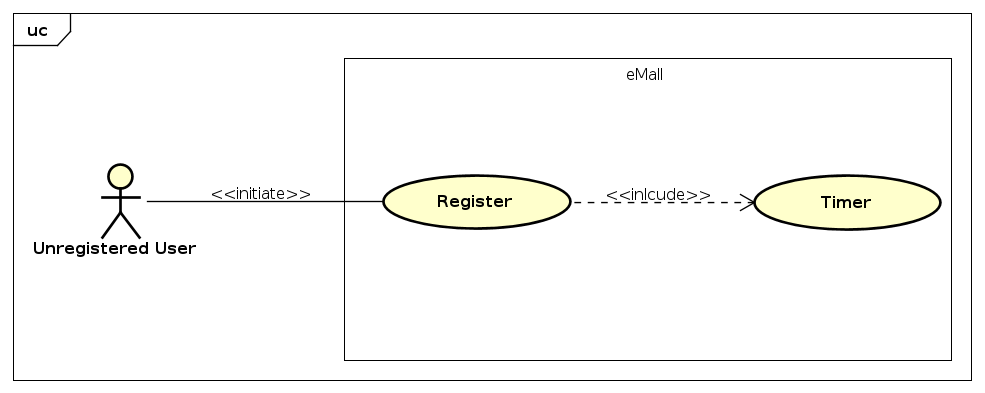
\includegraphics[keepaspectratio, width=16cm]{UseCase/UnregisteredUser.png}
    \caption{Unregistered user use case}
\end{figure}
\begin{figure}[!h]
    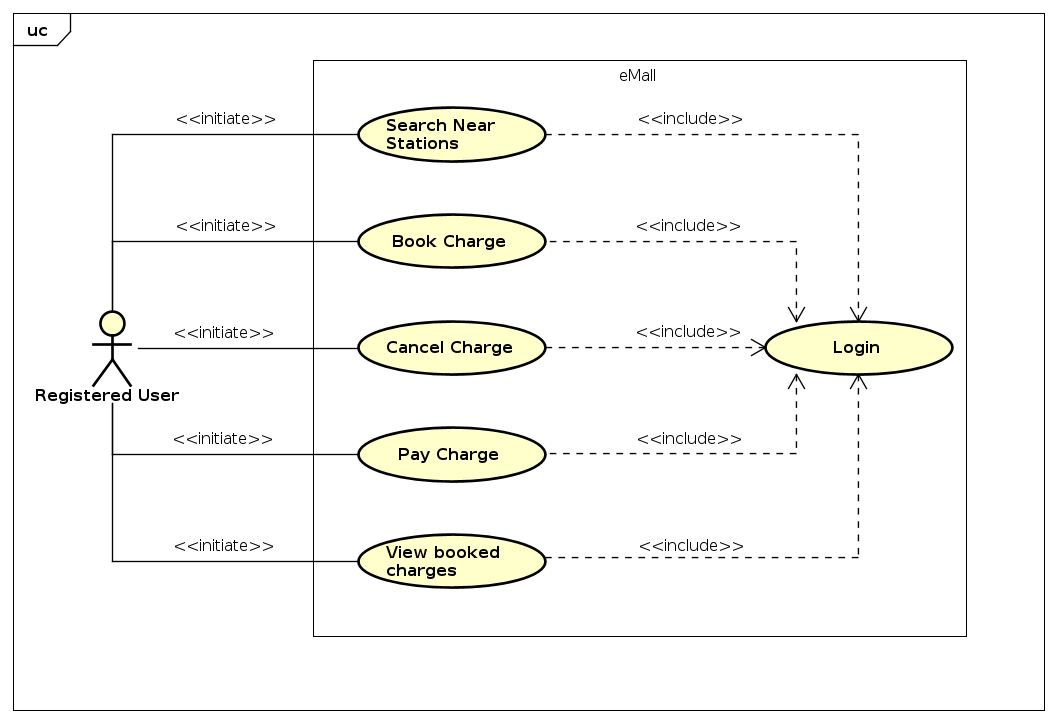
\includegraphics[keepaspectratio, width=16cm]{UseCase/RegisteredUser.png}
    \caption{Registered user use case}
\end{figure}
\begin{figure}[!h]
    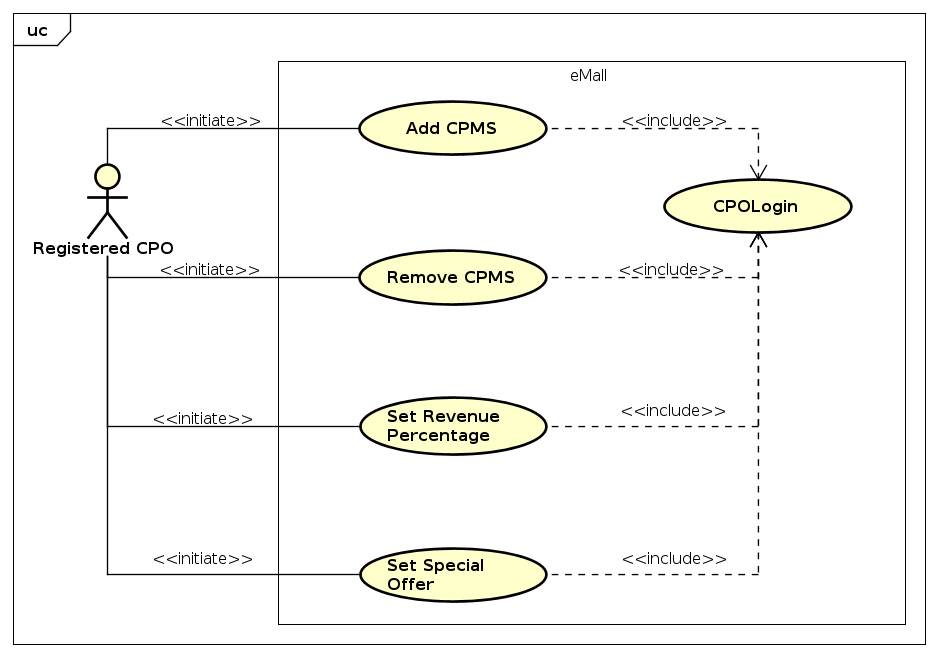
\includegraphics[keepaspectratio, width=16cm]{UseCase/RegisteredCPO.png}
    \caption{Registered \ac{CPO}}
\end{figure}
\begin{figure}[!h]
    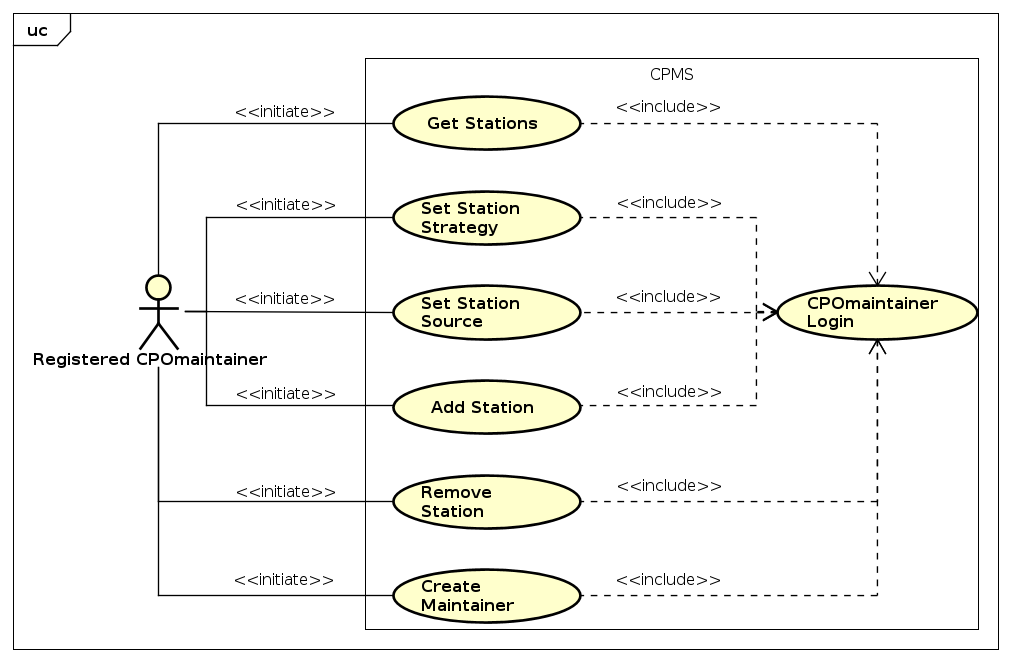
\includegraphics[keepaspectratio, width=16cm]{UseCase/RegisteredCPOmaintainer.png}
    \caption{Registered \ac{CPO}maintainer}
\end{figure}

\clearpage
\subsubsection{Sequence diagrams}
\begin{figure}[!h]
    \begin{center}
        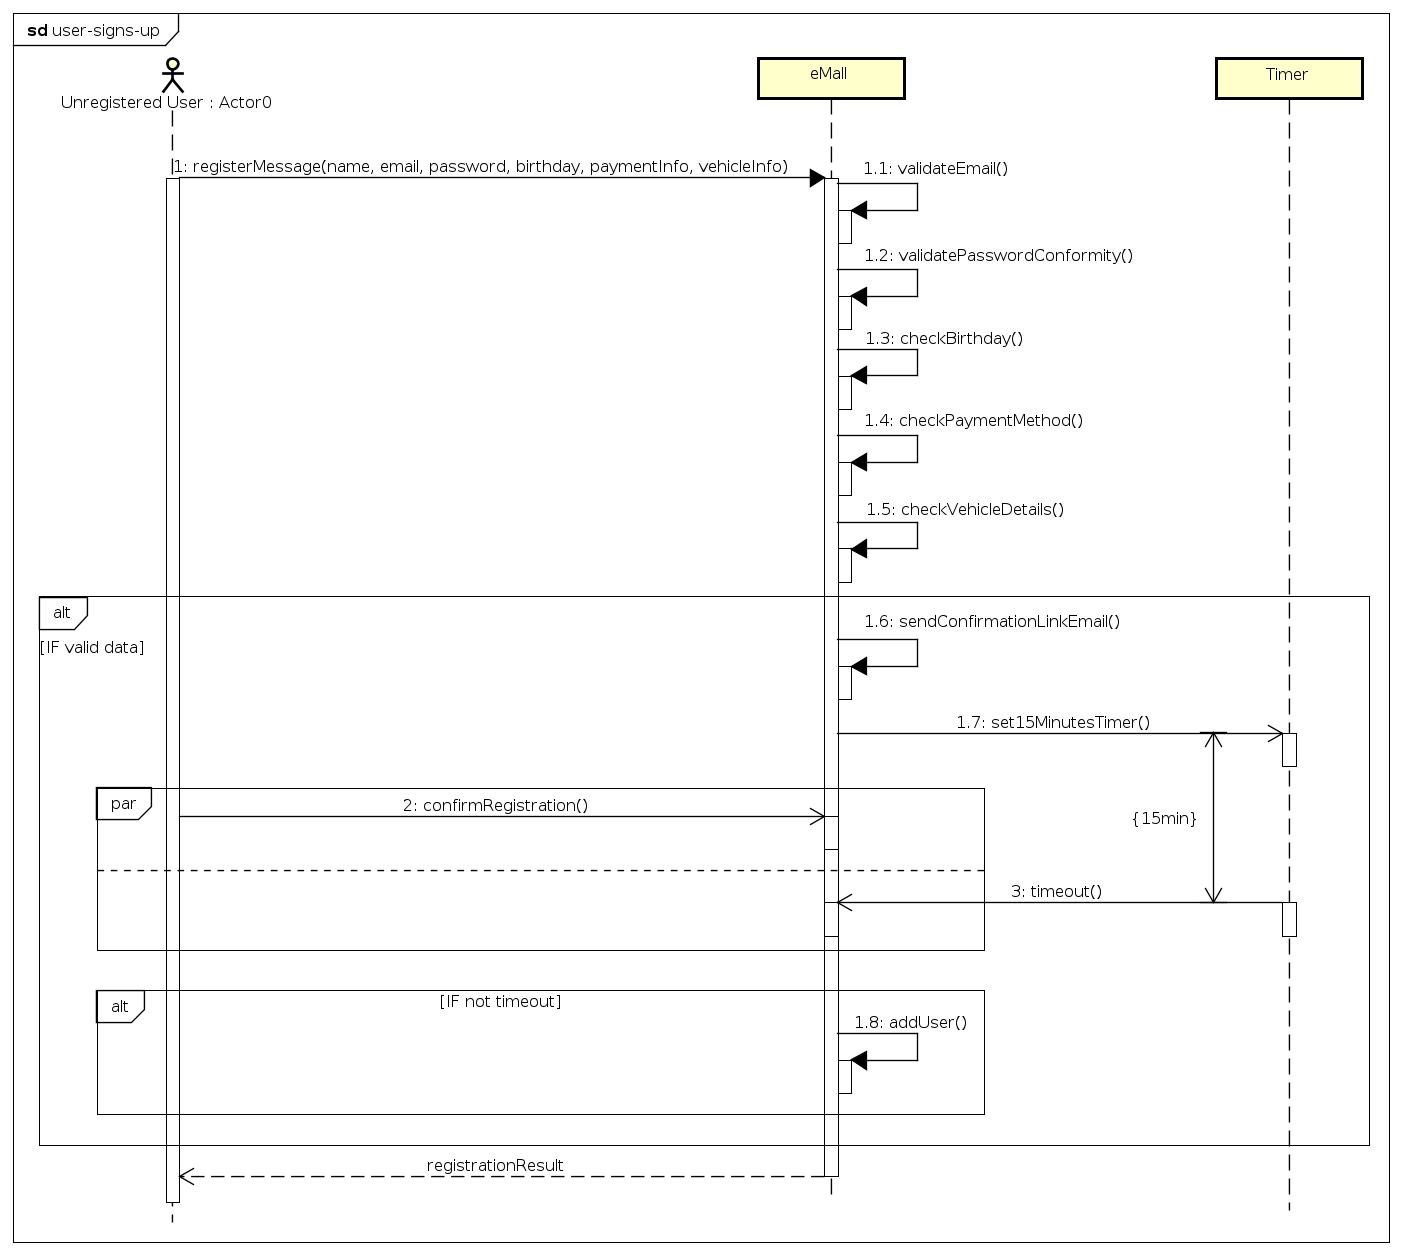
\includegraphics[keepaspectratio, width=16cm]{Sequence/user-signs-up.png}
        \caption{Registration into \ac{eMall} sequence}
    \end{center}
\end{figure}
\begin{figure}[!h]
    \begin{center}
        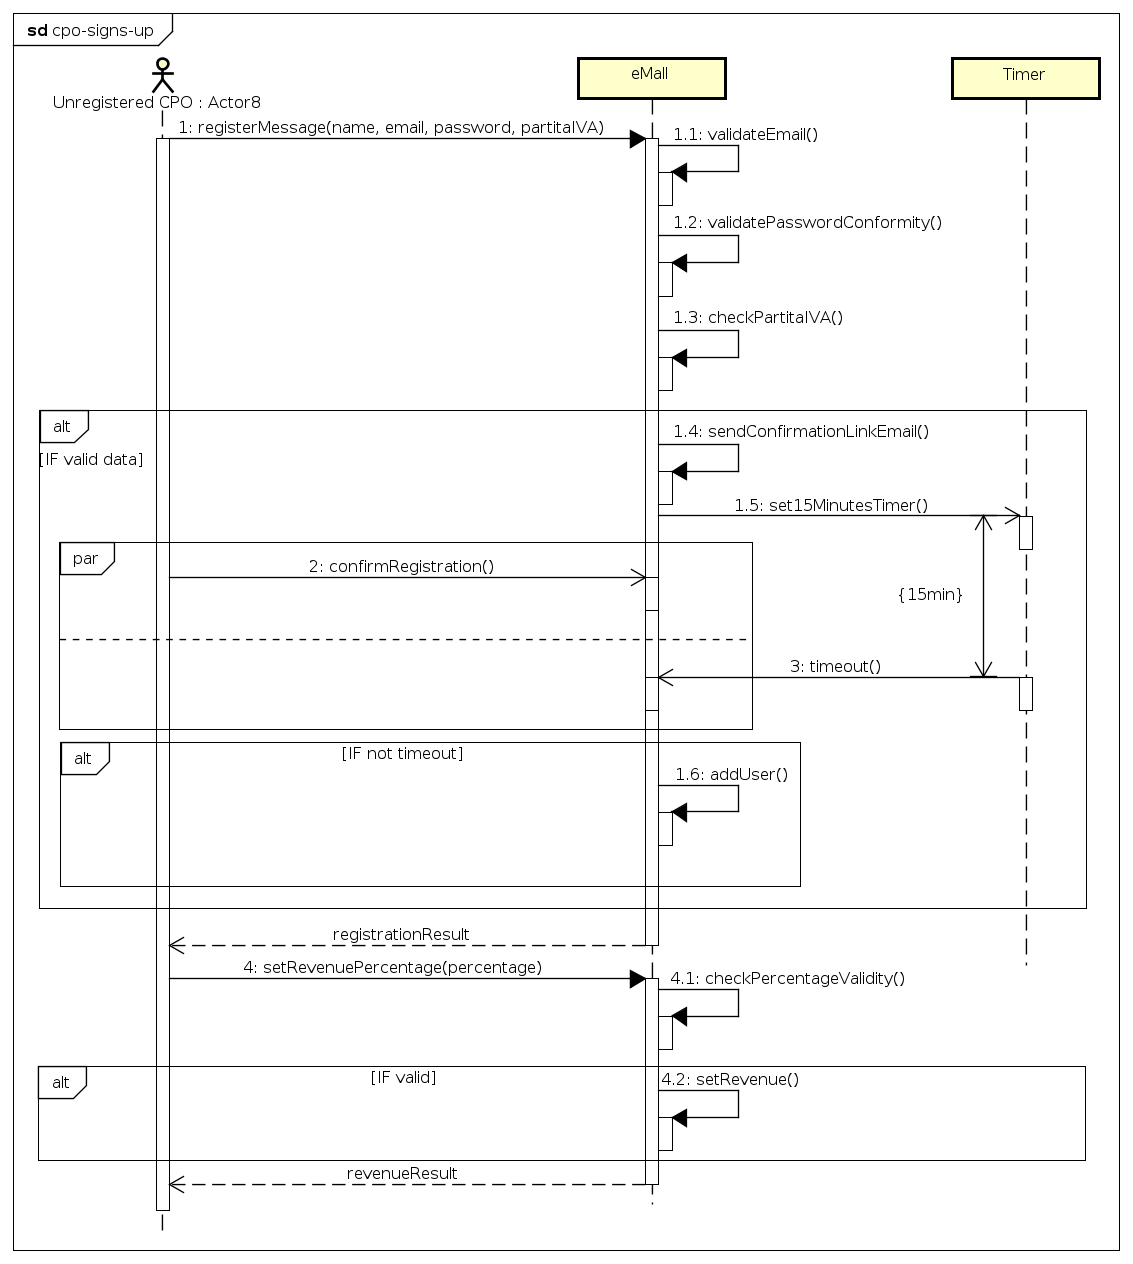
\includegraphics[keepaspectratio, width=16cm]{Sequence/cpo-signs-up.png}
        \caption{Registration of \ac{CPO} into \ac{eMall} sequence}
    \end{center}
\end{figure}
\begin{figure}[!h]
    \begin{center}
        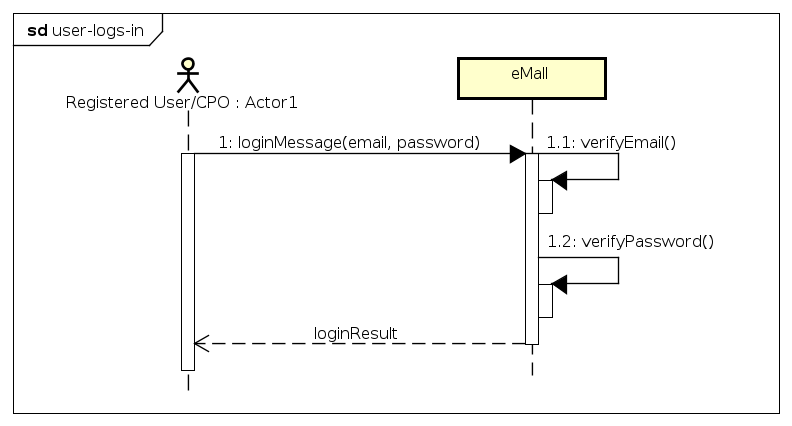
\includegraphics[keepaspectratio, width=16cm]{Sequence/user-logs-in.png}
        \caption{Login into \ac{eMall} sequence}
    \end{center}
\end{figure}
\begin{figure}[!h]
    \begin{center}
        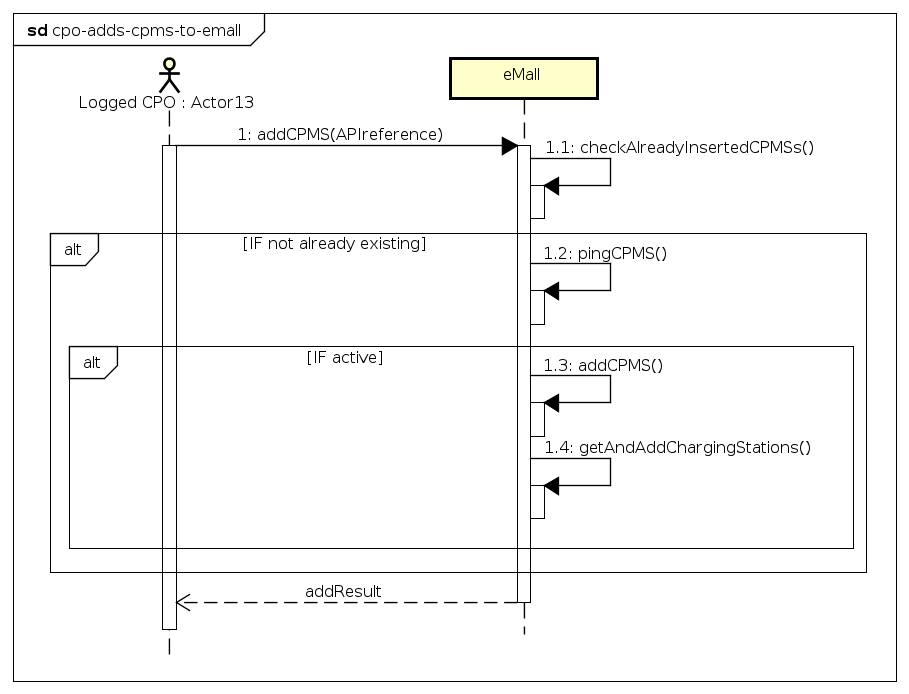
\includegraphics[keepaspectratio, width=16cm]{Sequence/cpo-adds-cpms-to-emall.png}
        \caption{\ac{CPO} adds a \ac{CPMS} into eMall}
    \end{center}
\end{figure}
\begin{figure}[!h]
    \begin{center}
        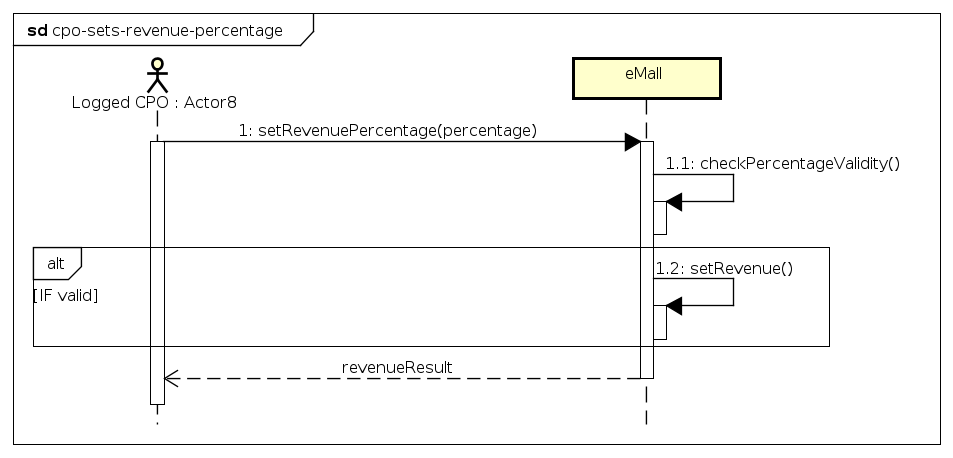
\includegraphics[keepaspectratio, width=16cm]{Sequence/cpo-sets-revenue-percentage.png}
        \caption{\ac{CPO} sets the revenue percentage}
    \end{center}
\end{figure}
\begin{figure}[!h]
    \begin{center}
        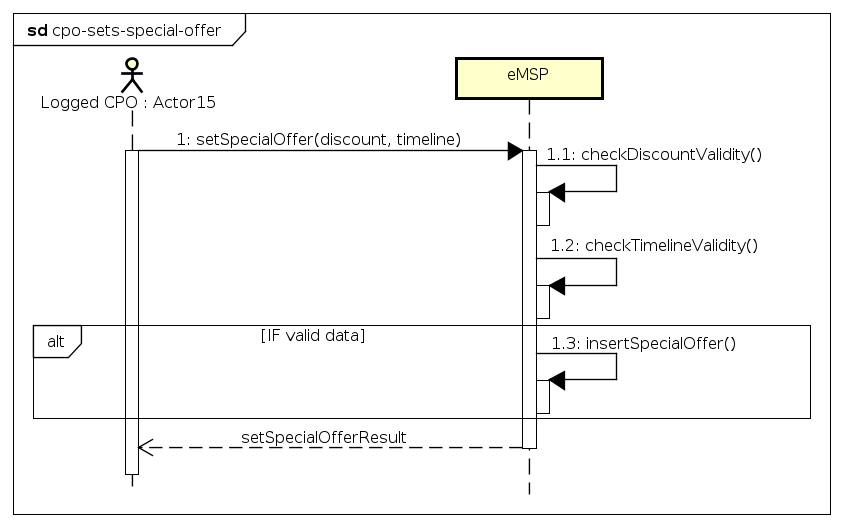
\includegraphics[keepaspectratio, width=16cm]{Sequence/cpo-sets-special-offer.png}
        \caption{\ac{CPO} sets a special offer}
    \end{center}
\end{figure}
\begin{figure}[!h]
    \begin{center}
        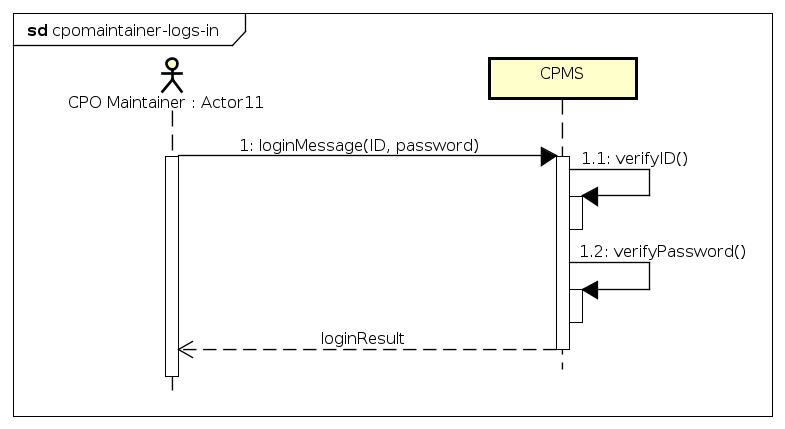
\includegraphics[keepaspectratio, width=16cm]{Sequence/cpomaintainer-logs-in.png}
        \caption{\ac{CPO} maintainer logs into \ac{CPMS}}
    \end{center}
\end{figure}
\begin{figure}[!h]
    \begin{center}
        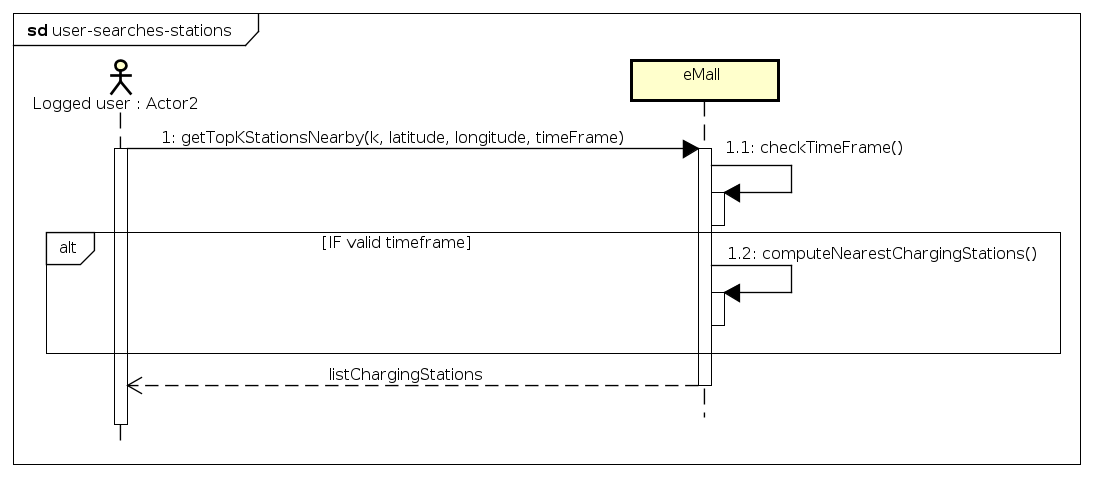
\includegraphics[keepaspectratio, width=16cm]{Sequence/user-searches-stations.png}
        \caption{Get the nearby charging stations}
    \end{center}
\end{figure}
\begin{figure}[!h]
    \begin{center}
        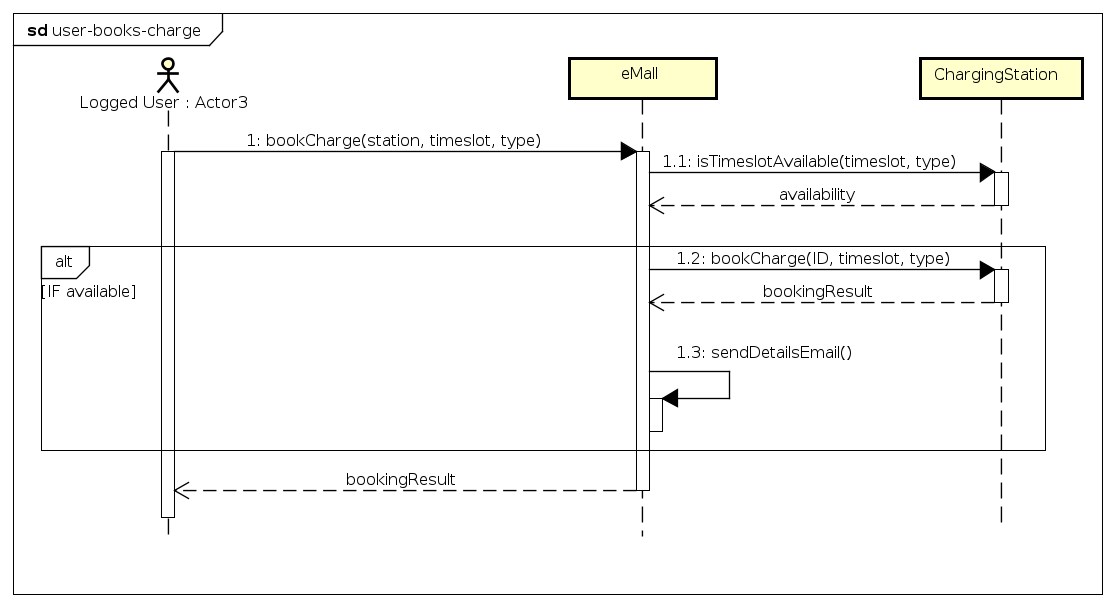
\includegraphics[keepaspectratio, width=16cm]{Sequence/user-books-charge.png}
        \caption{Book a charge sequence}
    \end{center}
\end{figure}
\begin{figure}[!h]
    \begin{center}
        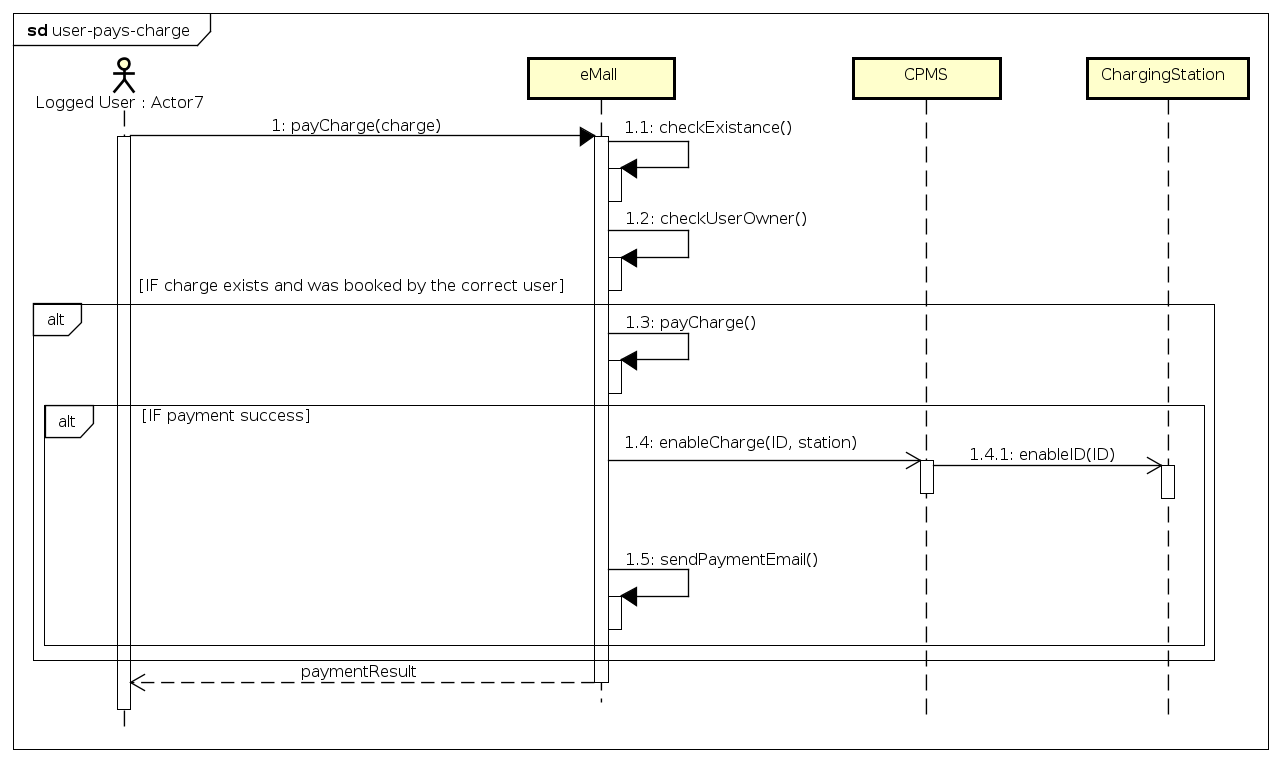
\includegraphics[keepaspectratio, width=16cm]{Sequence/user-pays-charge.png}
        \caption{Pay a charge sequence}
    \end{center}
\end{figure}
\begin{figure}[!h]
    \begin{center}
        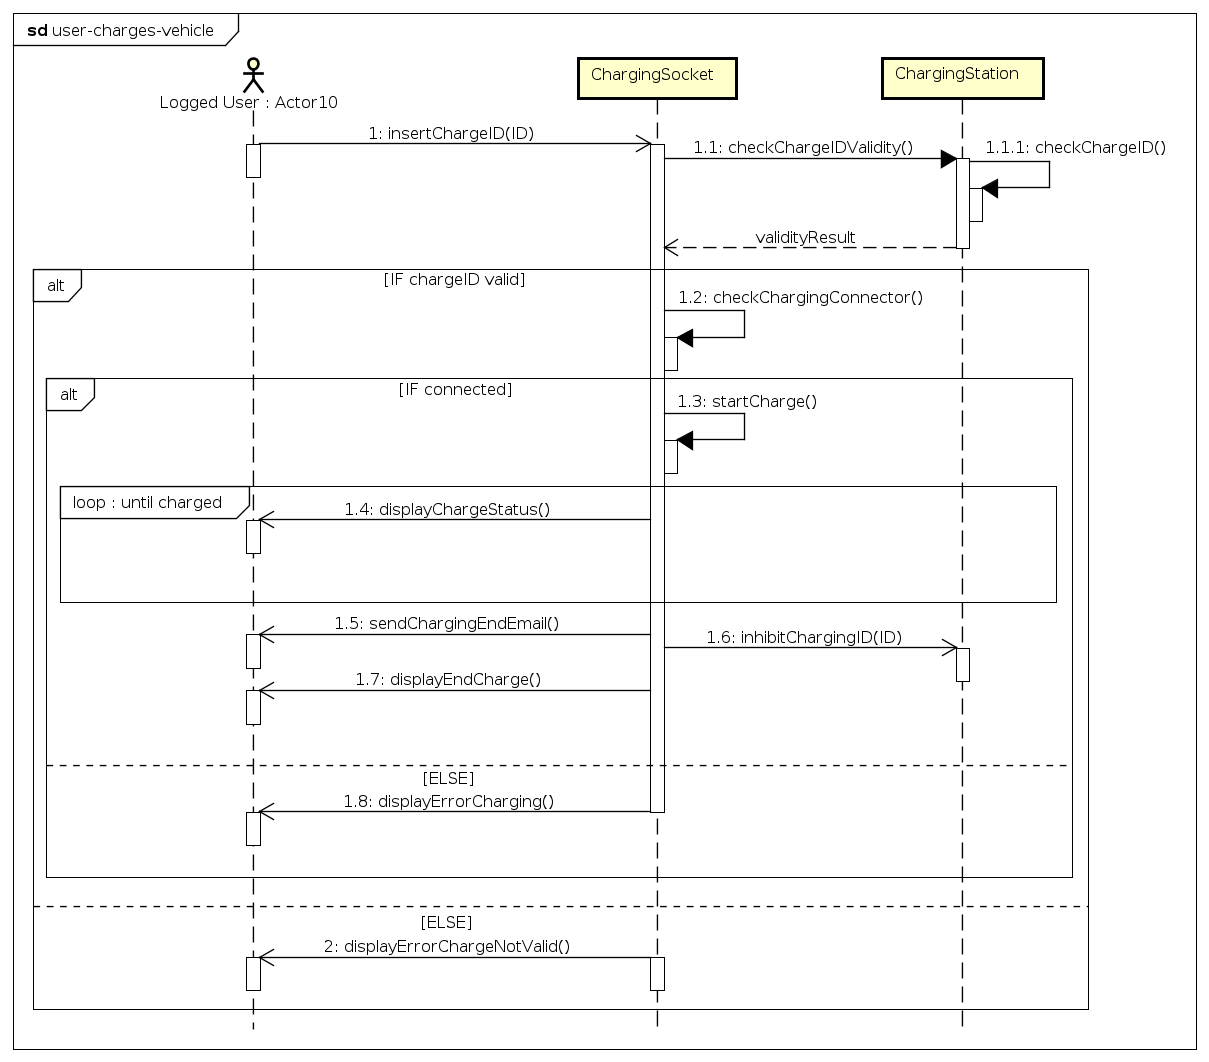
\includegraphics[keepaspectratio, width=16cm]{Sequence/user-charges-vehicle.png}
        \caption{Perform a charge sequence}
    \end{center}
\end{figure}
\begin{figure}[!h]
    \begin{center}
        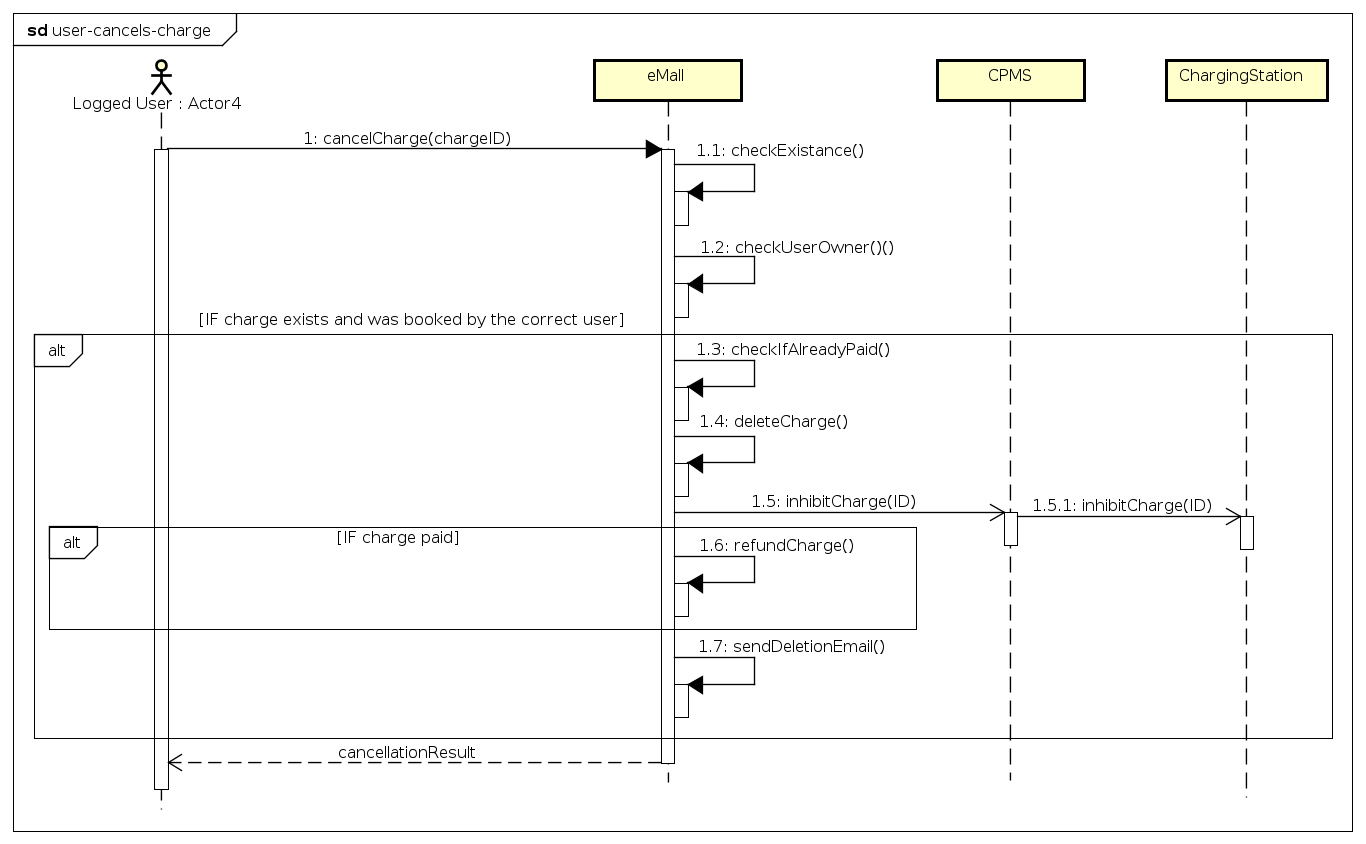
\includegraphics[keepaspectratio, width=16cm]{Sequence/user-cancels-charge.png}
        \caption{Cancel a charge sequence}
    \end{center}
\end{figure}
\begin{figure}[!h]
    \begin{center}
        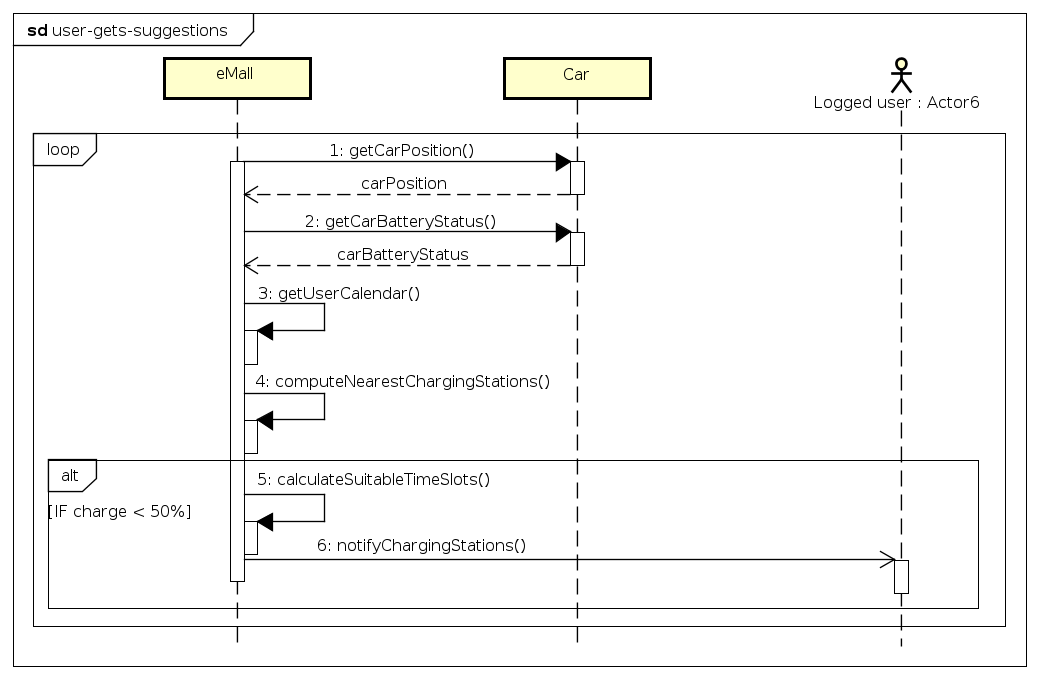
\includegraphics[keepaspectratio, width=16cm]{Sequence/user-gets-suggestions.png}
        \caption{Charging suggestions via calendar sequence}
    \end{center}
\end{figure}
\begin{figure}[!h]
    \begin{center}
        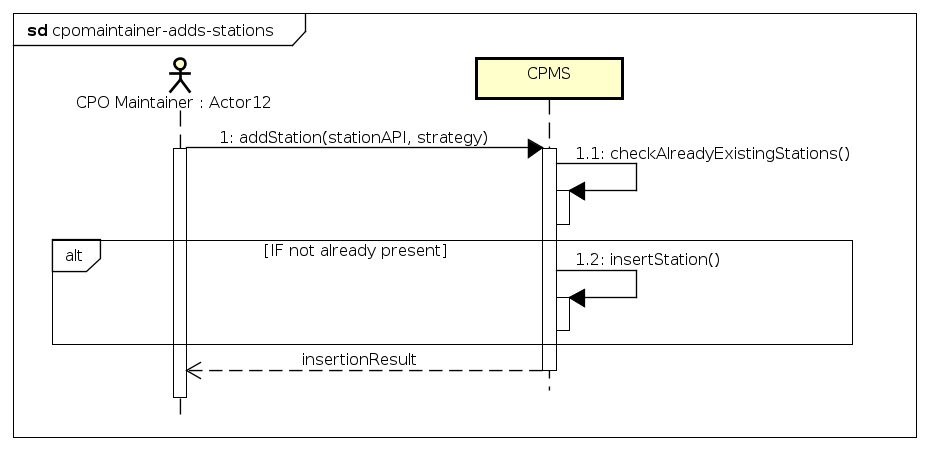
\includegraphics[keepaspectratio, width=16cm]{Sequence/cpomaintainer-adds-stations.png}
        \caption{\ac{CPO} maintainer adds stations to \ac{CPMS}}
    \end{center}
\end{figure}
\begin{figure}[!h]
    \begin{center}
        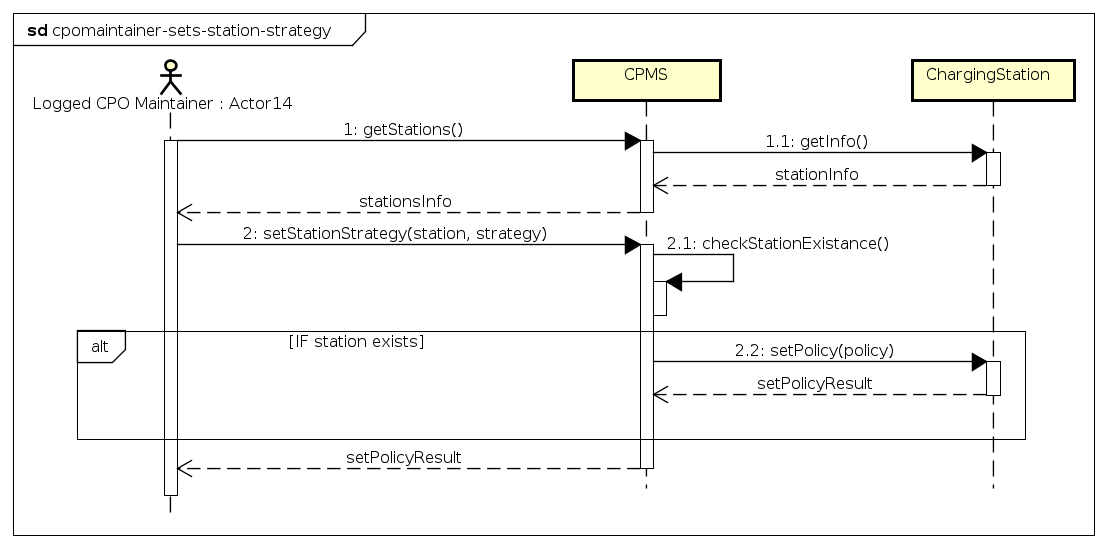
\includegraphics[keepaspectratio, width=16cm]{Sequence/cpomaintainer-sets-station-strategy.png}
        \caption{\ac{CPO} maintainer sets station strategy in \ac{CPMS}}
    \end{center}
\end{figure}

\begin{figure}[!h]
    \begin{center}
        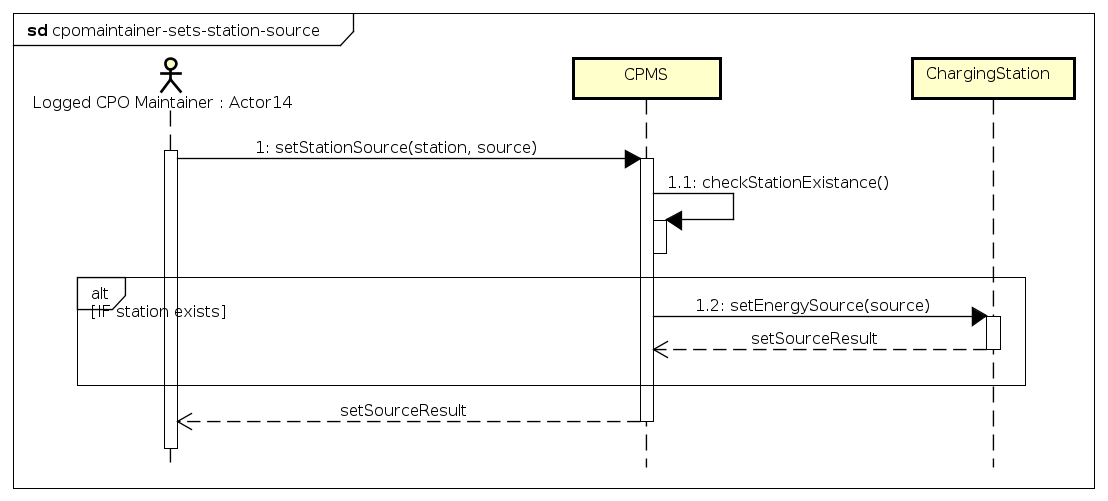
\includegraphics[keepaspectratio, width=16cm]{Sequence/cpomaintainer-sets-station-source.png}
        \caption{\ac{CPO} maintainer sets station source in \ac{CPMS}}
    \end{center}
\end{figure}

\clearpage
%Definition of use case diagrams, use cases and associated sequence/activity diagrams, and mapping on requirements
\subsection{Performance requirements}
The system in general needs to manage a large collection of electric vehicle users/\acp{CPO} and it needs to supply the heaviest services (like computing the cheapest nearest stations) in a reasonable amount of time.
Because of that the system shall guarantee a baseline load of 1000000 users/\acp{CPO} still with a response time not greater than 5 seconds. To achieve the goal, the system shall be able to decentralize all the computation as much as possible,
trying to make the client responsible of the heaviest loads.\\\\
These requirements are balanced considering the actual percentage of electric vehicle users in Italy [0.56\%] (corresponds to about 330k users) and a level of confidence of 3.
\subsection{Design constraints}
From this point we consider only the user side constraints as they represent the largest share of the system use base.
\subsubsection{Standards compliance}
The system must meet the following standards:
\begin{itemize}
    \item \textbf{\ac{GDPR} law}: The system must be compliant with the current GDPR law about users privacy;
    \item \textbf{Android and iOS}: The system must be compatible with the current versions and reasonably still used previous ones of Android and iOS.
\end{itemize}
\subsubsection{Hardware limitations}
Because the user side system consists of a smartphone app, the main hardware limitation is the computational capability of a smartphone processor. Hence the
application must be compatible with a low computational capability.

\subsection{Software system attributes}
\subsubsection{Reliability}
The system shall be fail safe, while the actual service can behave slower than expected it shall be still consistent with the results.
To do so the system shall be distributed data and performance wise, allowing a scalability factor while being open for maintenance without completely experiencing downtime.
Some good techniques are \ac{RACS} and \ac{RAPS} which put the reliability very high in the architecture.
\subsubsection{Availability}
Because a period of downtime would be detrimental, eMall has to prefer the availability over the conformity of response time.
Thus the availability should be as high as possible but greater than 99.99\% and must use some techniques to avoid down time during maintenance.
\subsubsection{Security}
Because the system will handle personal data, it has to abide the \ac{GDPR} law; thus an encryption of the user's password must be adopted and the access to the user's data must be restricted only to himself.
It is important that nobody else, not even the system administrator, can access the user's data in compliance of the privacy laws.\\
\subsubsection{Maintainability}
As stated in the Reliability and Availability sections, a good pattern for the whole system would be to consider the maintenance as less invasive as possible. Thus it would not be complicated to maintain a single or a restricted amount of nodes per time. This way the users would only experience at worst slowdowns but never downtime.
\subsubsection{Portability}
The system should be as cross platform as possible to increase the maintainability over different type of platforms.
\clearpage